\section{Aufbau}
\label{sec:Aufbau}

Die Messapparatur besteht aus einer Probe, die, wie in Abbildung \ref{fig:Aufbau} zu sehen, in eine Bleiabschirmung gesteckt wird, in der sich ein Zählrohr befindet, welches die durch die eintreffende Strahlung entstehenden Impulse über einen Verstärker an die Zähler weitergibt. Am Zeitgeber kann eingestellt werden wie lange die Messung laufen soll.
\begin{figure}
\centering
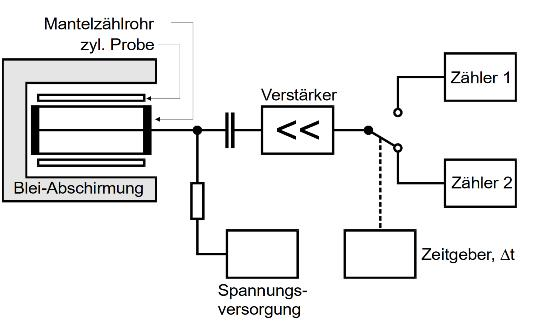
\includegraphics[scale=0.5]{content/images/aufbau.jpg}
\caption{Versuchsaufbau zur Bestimmung der Halbwertzeit radioaktiver Isotope \cite{V702}}
\label{fig:Aufbau}
\end{figure}